\documentclass[11pt,a4paper]{article}
\usepackage[T1]{fontenc}
\usepackage{lmodern}
\usepackage[margin=24mm,headheight=15pt,headsep=7mm]{geometry}
\usepackage{amsmath,amssymb,amsthm,booktabs,tabularx,array,graphicx,xcolor,fancyhdr}
\usepackage[colorlinks=true,linkcolor=blue!40!black,citecolor=blue!40!black,urlcolor=blue!40!black,breaklinks=true]{hyperref}
\definecolor{ink}{HTML}{243E55}
\pagestyle{fancy}\fancyhf{}\lhead{\small Tri-Octagon: geometric origins}\rhead{\small Local review draft v0.1}\cfoot{\thepage}
\setlength{\parindent}{0pt}\setlength{\parskip}{5pt}\setlength{\emergencystretch}{2em}\raggedbottom
\newcommand{\ph}{\varphi}\newcommand{\Li}{\operatorname{Li}}\newcommand{\conv}{\operatorname{conv}}
\newtheorem*{proposition}{Geometric consequence}
\hypersetup{pdftitle={Tri-Octagon: Geometric Origins, Normalization, and Constant Interpretations},pdfauthor={Hilmir Frimann Halldorsson},pdfsubject={GEO-ORIGINS-01 local manuscript review draft v0.1; not accepted for publication}}
\begin{document}
{\color{ink}\LARGE\bfseries Tri-Octagon: Geometric Origins,\par Normalization, and Constant Interpretations\par}
\vspace{4mm}
{\large Hilmir Fr\'imann Halld\'orsson}\par
17 October 2026 \quad GEO-ORIGINS-01 \quad Local review draft v0.1
\vspace{3mm}
\begin{abstract}
The folded Tri-Octagon has an exact geometry, while the images that motivated its construction have often been less explicit in the written record. This companion places the author's retrospective account beside the surviving definitions and accepted results. Opposite signs express an imagined other side; a unit expresses a normalization; neither alone specifies a physical sphere. The native shell nevertheless has a unique minimum enclosing ball. Extending its original straight lines gives two natural events: a whole unit-width chord at Crossing A and a unit-width addition at each endpoint at Crossing B. A also circumscribes the earlier measurement cylinder and triangular-prism envelope, and its endpoint addition equals the shortest native notch gap. We trace the historical resonance-lock proposal through the fixed target $\gamma_*$ and the exact golden-interval zeta identity. These connections are retained without conflating layer counts, analytic coefficients, assigned spatial units and an as-yet unspecified structural extent.
\end{abstract}

\section{The construction picture and its surviving record}
Hilmir describes the early work with GPT-4o as a sustained collaboration. In his account of 17 October 2026, the original conversations had been deleted, while the papers survived. Equations were retained more consistently than the geometric thinking that led to them. The purpose here is to place that thinking back beside the mathematics. The account supplies the author's motivation; the surviving documents supply the equation record. Missing conversations do not imply missing intuition, and they do not allow exact per-equation contributions or dates of discovery to be reconstructed.~\cite{Intent,Collab}

One motivating image places a reference universe at $1$ and an imagined counterpart at $-1$. The author explicitly says this does not express a belief in a mirror universe: the opposite sign pictures another side of a toroidal construction. His analogy of turning a two-dimensional map horizontally through $180^\circ$ conveys the desire to see a fuller three-dimensional picture. No particular axis, sweep surface or map from that image to the welded module was specified. A coordinate may be signed while a Euclidean distance remains nonnegative; for example, positions $-1$ and $1$ on a coordinate axis have distance $2$ in that coordinate unit. This illustrates the distinction, without identifying either position with a shell vertex.~\cite{Intent}

Asked whether an invisible surrounding sphere was part of the original picture, the author answered no. The later exact enclosing sphere is therefore a consequence of the specified geometry, not evidence that this sphere was consciously assumed at the start. Similarly, toroidal imagination and toroidal topology are different matters. The accepted welded shell has three octagonal faces, eighteen vertices, twenty-one unique edges and two open nine-edge rims. Its Euler characteristic is zero and its orientable surface has two boundary components, so it is an annulus. Paper C establishes this topology rather than inferring a torus from the word ``toroidal.''\cite{PC,SP}

The author's further picture treats $\pi$, $e$ and $\ph$ as base or boundary-structure constants, and other constants as descriptors of structures ``above'' them. That is a proposed organization of roles, not an ordering of numerical magnitudes. His accompanying uncertainty about ``base one'' and ``fuller ten'' is part of the account. The useful question is how a chosen unit and a proposed extent would be represented by named mathematical quantities. The following sections begin with the constructions that already have such names.~\cite{Intent}

\section{Circles, half units and the meaning of a size}
The author's Vesica picture combines a unit size, a half-radius displacement, an eye-like circle and a half-$\pi$ relation. Those ideas can be set beside the actual conventions without forcing them into a single definition. In the February 2025 VPQW paper, the Gaussian centres are
\begin{equation}\label{eq:centres}
c_- =(-r/2,0),\qquad c_+=(r/2,0),\qquad \|c_+-c_-\|=r.
\end{equation}
Thus each centre has a half-radius offset from their midpoint; their total separation is a full radius. The March paper repeats these centre labels in Figure 1. A total separation $r/2$ would be another configuration. Neither the phrase ``Vesica size one'' nor the offsets alone identify whether the unit is a parent-circle diameter, lens width or another construction variable.~\cite[Sec.~5.2, p.~3]{VPQW}~\cite[Fig.~1; Sec.~2]{Fractal}

The \emph{Vesica Delay Method} supplies a different explicit half-unit convention: parent radius $r=1/2$ and
\begin{equation}\label{eq:vesica}
d=2r\cos\theta,\qquad C_{\rm overlap}=4r\theta,
\qquad 0\leq\theta\leq\pi/2.
\end{equation}
For two equal disks this perimeter consists of two circular arcs, each of angle $2\theta$. At $\theta=\pi/4$, it is $\pi/2$; at coincidence, $\theta=\pi/2$ and $d=0$, it is $\pi$. This is a precise half-$\pi$ relationship between two configurations. The nondegenerate lens at $d>0$ has arcs with different centres and is not a circle. An associated eye-circle may have a separate role in the author's image, but no map identifying it with the whole lens or the Tri-Octagon sphere has been supplied.~\cite[p.~1, Eqs.~(1)--(2)]{Delay}

\begin{figure}[htbp]\centering
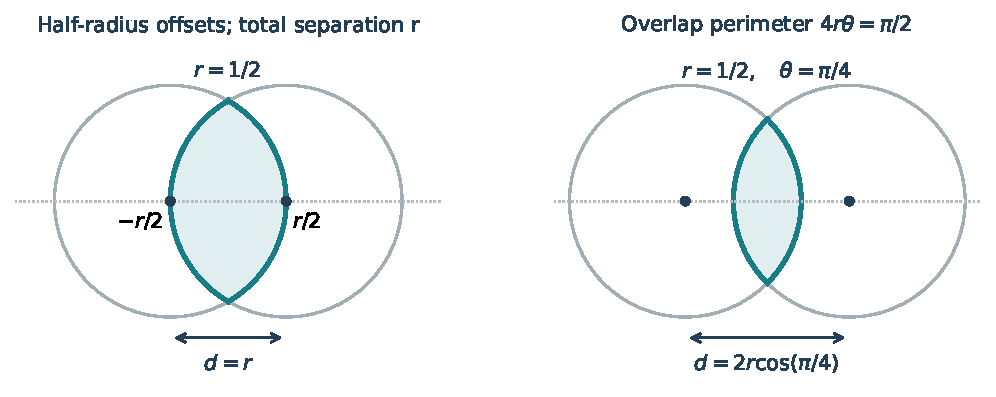
\includegraphics[width=\linewidth]{figures/circle_conventions.pdf}
\caption{Two explicit circle constructions, drawn from their stated equations. Left: centres displaced by $\pm r/2$ have separation $r$. Right: the Delay Method's $r=1/2$, $\theta=\pi/4$ gives overlap perimeter $\pi/2$. These are deterministic geometric schematics, not a proposed quantum state or a reconstruction of an undocumented eye-circle.}\label{fig:circles}
\end{figure}

A surviving inconsistency matters to this history. Both early quantum documents print $C=\pi$ together with $r=1/(2\pi)$. Under the ordinary circle equation $C=2\pi r$, the first statement instead gives $r=1/2$, while the printed radius gives $C=1$. We retain the two printed statements as a source inconsistency; the consistent $r=1/2$ in the later Delay Method does not silently repair them.~\cite[Sec.~5.1, pp.~2--3]{VPQW}~\cite[Sec.~2.1, p.~2]{Fractal}

The VPQW golden-ratio expression in Sec.~6.2 is an algebraic identity involving $\ph/\sqrt3$; the March paper explicitly defers deeper golden-ratio detail in Sec.~3. These recovered passages do not derive $\rho/w=\ph-1$. The particular derivation remembered by the author may be another source; its exact equation remains unrecovered. The geometric statements used here do not certify the quantum or perceptual interpretations accompanying them.

\section{The documented unit and the exact welded module}
The author's wish to work with a reference value of one has a precise implementation in the construction record. Specification v0.1 used octagon edge $s=1$. Specification v0.2 records an author-requested change to flat-to-flat panel width $w=1$, preserving placement, connectivity and angles. For arbitrary width $w>0$,
\begin{equation}\label{eq:normalization}
s=(\sqrt2-1)w,\qquad h=s/2,\qquad
w_{s=1}=1+\sqrt2,\qquad q=\sqrt2-1.
\end{equation}
Multiplying the old coordinates by $q$ gives $q(1+\sqrt2)=1$: this is the documented edge-one to width-one normalization. Lengths scale by $q$ and areas by $q^2$. It is not a documented division by ten. The recollection of a reduction by ten can remain a comparison idea without replacing the recorded normalization.~\cite{Spec1,Spec2}

Hereafter $w$ always denotes \emph{panel flat-to-flat width}. In local panel coordinates $(u,z)$, the eight vertices are $(\pm w/2,\pm h)$ and $(\pm h,\pm w/2)$, with independent signs. Place the panels vertically on the three side planes of an equilateral triangle $K$ of side $w$, with each panel centred at the midpoint of its side. In centred horizontal coordinates one may take
\begin{equation}\label{eq:triangle}
K=\conv\left\{(0,a),\ (w/2,-a/2),\ (-w/2,-a/2)\right\},
\qquad a=\frac{w}{\sqrt3}.
\end{equation}
The adjacent vertical edges coincide at the three triangle corners for $|z|\leq h$. This is the accepted folded realization, up to rigid choice of frame. In Paper C's global frame its centre is $o=(0,\sqrt3w/6,0)$; we use $X=x-o$. The interior dihedral angle is $60^\circ$, while the outward-normal angle is $120^\circ$. A static final realization is specified; no collision-free folding path is inferred.~\cite[Secs.~2--5, 7]{PC}~\cite[Sec.~2]{SP}

The three filled, zero-thickness panels form the native shell $S$. Their edges are finite segments. Their infinite supporting lines form another object. A sphere of radius $R$ clips those lines into a framework, and the convex hull of their outer exits forms an envelope. An observation surface is not a new panel, and an envelope does not supply a material wall. These distinctions give the construction image a precise vocabulary without requiring a physical interpretation.

\section{The spheres fixed by the geometry}
Each panel plane is at distance $p=w/(2\sqrt3)$ from the centre. Its local circumradius satisfies $R_8^2=w^2/4+h^2$. Perpendicular decomposition therefore gives the common vertex radius
\begin{equation}\label{eq:rho}
\rho^2=p^2+R_8^2
=w^2\left(\frac{13}{12}-\frac{\sqrt2}{2}\right),
\qquad \rho/w\approx0.613373093758428410 .
\end{equation}
This makes an implicit enclosing sphere available even though it was not part of the original mental picture. It is also the \emph{unique minimum enclosing ball}, not merely one convenient sphere. To recall the accepted proof, the eighteen centred vertices have mean zero and common squared norm $\rho^2$. For any alternative centre $c$,
\begin{equation}\label{eq:minball}
\frac1{18}\sum_i\|X_i-c\|^2=\rho^2+\|c\|^2.
\end{equation}
An enclosing ball must have squared radius at least this mean. The centre $c=0$ attains $\rho$; every other centre requires a larger radius. Convexity of a ball extends containment from vertices to each panel, all finite edges and their convex hull. This restates the BOUNDARY-10 proof retained in the accepted synthesis.~\cite[Sec.~3]{SP}

There is a second intrinsic sphere. For an edge with midpoint $m$ and half-edge vector $D$, equal endpoint norms imply
\begin{equation}\label{eq:midpoint}
m\mathbin{\cdot}D=0,\qquad \|D\|=h,\qquad
\|m\|^2=\rho^2-h^2=\frac{w^2}{3}=a^2.
\end{equation}
Writing $u=D/h$, the supporting line obeys $\|m+tu\|^2=a^2+t^2$. It is tangent to the radius-$a$ sphere at its midpoint. This sphere does not enclose the shell and is not its face-tangent insphere: the panel planes are only distance $p=a/2$ from the centre. Thus ``a surrounding sphere'' and ``the edge-tangent sphere'' answer different questions.~\cite[Sec.~3]{SP}

The nearby golden-ratio comparison can now be written with its two meanings visible:
\begin{equation}\label{eq:golden-gap}
\ph-1\approx0.618033988749894848,\qquad
(\ph-1)-\rho/w\approx0.004660894991466438 .
\end{equation}
The author's recollected association is a motivation to seek a map, not an equality between these numbers. No resizing or rounding of the accepted shell is needed. A transformation relating their roles would have to be stated separately.~\cite{Intent,TSZReview}

\section{Two natural completions of the straight edges}
The wish to see a fuller outer construction acquires a precise static form by extending each original edge along its own line. For an observer sphere $R\geq\rho$, its exits are
\begin{equation}\label{eq:line}
q^{\pm}(R)=m\pm tu,\qquad t=\sqrt{R^2-a^2},\qquad
C=2t,\quad \ell=t-h.
\end{equation}
Here $C$ is the whole sphere-to-sphere segment and $\ell$ is the added distance at \emph{each} endpoint. The accepted incidence classification gives, on every outward ray, the first subsequent supporting-line meeting at $t_A=w/2$ and the last finite meeting at $t_B=(1+\sqrt2)w/2$. These are incidence-defined stopping rules; $R$ is not time. Their immediate length consequences are
\begin{equation}\label{eq:units}
C_A=w,\qquad \ell_A=\left(1-\frac{\sqrt2}{2}\right)w,
\qquad C_B=(1+\sqrt2)w,\qquad \ell_B=w.
\end{equation}
Thus one unit appears as a \emph{whole chord} at A and as an \emph{added endpoint extension} at B. Combining the same line equation with $a^2=w^2/3$ gives
\begin{equation}\label{eq:events}
\frac{R_A}{w}=\sqrt{\frac7{12}},\qquad
\frac{R_B}{w}=\sqrt{\frac{13}{12}+\frac{\sqrt2}{2}}.
\end{equation}
No constant target was used to locate these events. At Original, A and B, forty-two branch labels occupy eighteen distinct outer points; other allowed finite radii have forty-two distinct exits. Splitting at spatial intersections gives the frameworks below, while convexification gives different edge and face counts.~\cite[Secs.~5, 8--10]{SP}

\begin{table}[htbp]\centering\small
\caption{Accepted event geometry at common width $w$; decimals are rounded. A framework includes interior intersections; its envelope is a separate convex polyhedron.}\label{tab:events}
\begin{tabular}{@{}lccc@{}}\toprule
 & Original & Crossing A & Crossing B\\\midrule
Radius $R/w$ & $0.613373094$ & $0.763762616$ & $1.338073284$\\
Whole chord $C/w$ & $\sqrt2-1$ & $1$ & $1+\sqrt2$\\
Per-end addition $\ell/w$ & $0$ & $1-\sqrt2/2$ & $1$\\
Framework $(V,E)$ & $(18,21)$ & $(36,63)$ & $(54,105)$\\
Hull $(V,E,F)$ & $(18,27,11)$ & $(18,48,32)$ & $(18,36,20)$\\\bottomrule
\end{tabular}
\end{table}

\subsection{Why the measurement enclosure reaches A}
The earlier measurement construction uses a vertical cylinder of radius $a=w/\sqrt3$ and half-height $w/2$. Its two rim circles lie on the sphere
\begin{equation}\label{eq:cylinder}
R_{\rm cyl}^2=a^2+(w/2)^2=\frac7{12}w^2=R_A^2.
\end{equation}
The triangular-prism envelope $K\times[-w/2,w/2]$ has six corners with that same radius and mean zero. The mean-square argument in \eqref{eq:minball} forces its unique minimum ball; the ball also contains the whole cylinder, whose rim circles attain its radius. The six prism corners are precisely the A exits of the three seam lines. This is the accepted cross-source connection between measurement geometry and first line meetings.~\cite{TSZSphere,TSZReview}

The full A framework is larger in different directions: its other exits include $z=\pm w/\sqrt2$, and its six equatorial exits have horizontal radius $R_A>a$. Hence the A framework is neither the cylinder nor the prism, despite their shared circumsphere. The original shell is smaller still because it does not attain horizontal radius $a$ and height $w/2$ simultaneously. Shared enclosing radius is the exact correspondence, rather than equality of sets.

\begin{figure}[htbp]\centering
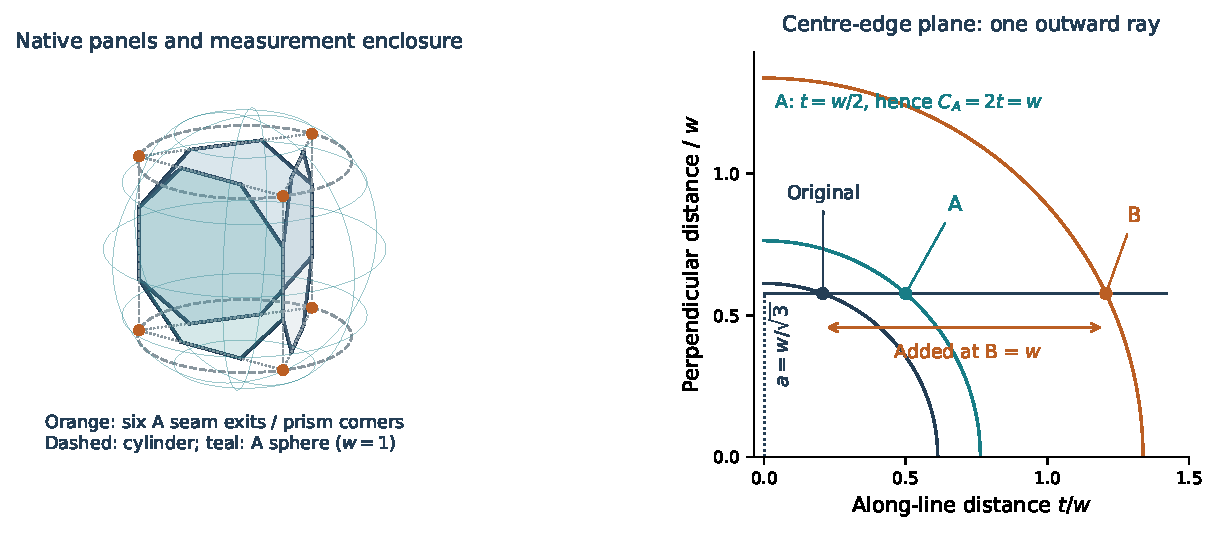
\includegraphics[width=\linewidth]{figures/shell_and_lengths.pdf}
\caption{Left: the accepted eighteen-vertex shell at $w=1$, the measurement cylinder/prism and their A circumsphere. Only the six A seam exits are highlighted; the complete A framework is not depicted as the prism. Right: a plane through the centre and one edge line. Circular sections show Original, A and B at one common scale. The horizontal addition at B is $w$; the A half-chord is $w/2$. Stored native coordinates and stated formulas were rendered deterministically, without a new geometry solve.}\label{fig:shell}
\end{figure}

There is another exact bridge to the original shape. The retained TSZ vertex-distance classification gives the shortest native vertex gap as six rim-notch chords with squared length $(3/2-\sqrt2)w^2$. Since
\begin{equation}\label{eq:notch}
\left(1-\frac{\sqrt2}{2}\right)^2=\frac32-\sqrt2,
\qquad 1-\frac{\sqrt2}{2}>0,
\end{equation}
their length is exactly $\ell_A$. These chords are shorter than the original edges and are not additional welded edges. This equality, explicitly explained in GPT's accepted TSZ review, reuses the distance and event results; it is not a new classification or a claim of global novelty.~\cite{TSZAtlas,TSZReview}

\section{The historical lock, the exact target and the roles of ten}
The author's association of constants with structure preceded this sphere comparison. In particular, $T$ was not selected by inspecting Crossing B. The September 2025 URF manuscript describes a resonance-lock coupling $\gamma$, inferred from a run's spectra and adjusted toward
\begin{equation}\label{eq:lock}
\pi e\ph\approx\gamma^{-1}\zeta(3).
\end{equation}
Its pages 8--9 call $\gamma$ emergent and run-dependent. Geometry--Zeta Investigation 01, dated 9 October 2026, then distinguishes the exact fixed target
\begin{equation}\label{eq:target}
\gamma_*:=\frac{\zeta(3)}{\pi e\ph},\qquad
T:=\frac{\zeta(3)}{\gamma_*}=\pi e\ph
\approx13.817580227176494440 .
\end{equation}
The target is a definition, the historical coupling is a proposed estimator, and Euler--Mascheroni's constant $\gamma_{\rm EM}$ is a third quantity. The exact target does not retroactively turn every historical coupling estimate into its value. The accepted spherical synthesis preserves this chain in Eqs.~(25)--(26), printed p.~18 (physical PDF p.~20), with source distinctions in Appendix E.~\cite[pp.~8--9]{URF}~\cite[Sec.~1]{GZ}~\cite[Sec.~14; App.~E]{SP}

\subsection{An analytic ten, not a selected radius}
With $L=\ln\ph$, the already recorded golden-interval identity is
\begin{equation}\label{eq:integral}
I_2:=\int_0^L x^2\coth x\,dx=\frac{\zeta(3)}{10},
\qquad \frac{T}{10}=\frac{I_2}{\gamma_*}.
\end{equation}
The integral is dimensionless; $x^2\coth x\sim x$ at zero, so its lower endpoint is finite. To display the inherited algebra, put $q=\ph^{-1}$ and use $q+q^2=1$. Expanding $\coth x=1+2\sum_{n\geq1}e^{-2nx}$ and integrating the nonnegative series gives
\begin{equation}\label{eq:polylog}
I_2=\frac{L^3}{3}+\frac{\zeta(3)}2
-\frac{\Li_3(q^2)}2-L\Li_2(q^2)-L^2\Li_1(q^2).
\end{equation}
The classical golden values used in the accepted derivation are
\begin{align}
\Li_1(q^2)&=L,&\Li_2(q^2)&=\pi^2/15-L^2,\notag\\
\Li_3(q^2)&=\tfrac45\zeta(3)-\tfrac{2\pi^2L}{15}+\tfrac23L^3.\label{eq:golden-polylogs}
\end{align}
Substitution cancels the $L^3$ and $\pi^2L$ terms, leaving $(1/2-2/5)\zeta(3)=\zeta(3)/10$. These are inherited analytic identities, with their proof and Hjortnaes/Markov attribution retained in the cited sources, not discoveries of this companion. The second equality in \eqref{eq:integral} then follows by division by the defined $\gamma_*$. It does not independently select a shell width.~\cite[Sec.~7]{GZ}~\cite[App.~E, printed pp.~24--25]{SP}

The same Geometry--Zeta note separates a spectrum-generated numerator from an adopted normalization. Its auxiliary unit-circumference cycle, for $N\geq3$, has eigenvalues $\lambda_{N,k}=4N^2\sin^2(\pi k/N)$. The zero mode is omitted, and for $\alpha>1/2$ it proves
\begin{equation}\label{eq:spectrum}
Z_N(\alpha)=\sum_{k=1}^{N-1}\lambda_{N,k}^{-\alpha}
\longrightarrow\frac{2\zeta(2\alpha)}{(2\pi)^{2\alpha}}.
\end{equation}
At $\alpha=3/2$ the limit is $\zeta(3)/(4\pi^3)$; multiplying by $4\pi^2/(e\ph)$ gives $\gamma_*$. That multiplier inserts the chosen target normalization. The full-cycle spectrum, its zero-mode policy and its inverse moment are explicit additional choices, not a native shell energy law. The note's finite-part energy-type observable is different again.~\cite[Secs.~3--6]{GZ}

\subsection{Ten as structure, count and convention}
Hilmir supplied the June 2025 recursive-toroidal compilation as a reason for choosing ten. Its physical/printed p.~11 explicitly specifies $N=10$ layers in a model of nested toroidal shells. Pages 7--8 group $\pi,e,\ph$ within a ``Stable Harmonic Core'' and Ap\'ery's $\zeta(3)$ within ``Deep Recursive Excitations''; p.~12 repeats their separation in a later phase classification. These are reported interpretations of that historical study; its simulations and classifications are not revalidated here. The author's present picture extends beyond the layer count: base one and fuller ten suggest a possible extent of an organized whole. His uncertainty about what that extent measures remains explicit.~\cite{Toroidal,Intent}

Several distinct tens therefore coexist. The $10$ in \eqref{eq:integral} is an analytic coefficient; $N=10$ counts layers. The accepted source ledger also records a historical real-space box-length parameter of ten, without a map to the Tri-Octagon. An assigned observer value such as $R/w=10$ is yet another convention. Finally, ``full size ten'' is a proposed structural or tensor extent, whose measure and norm are not specified. The exact recalled aggregate of constants approaching ten has not been recovered. Keeping these roles separate retains the motivation while leaving a concrete place for the missing relation.~\cite[Sec.~14; App.~E]{SP}~\cite{Intent,TSZReview}

\section{What the retained numerical comparisons establish}
Let $b=R_B/w=\sqrt{13/12+\sqrt2/2}$. TSZ examined the explicit counterfactual $w=10U$, with a target \emph{radius} $TU$ in an arbitrary common length unit $U$. Then the dimensional radial gap is $DU$, where
\begin{align}
D&:=T-10b\approx0.436847382821963879,\label{eq:D}\\
D-5\gamma_*&\approx0.001873645236788866 .\label{eq:mismatch}
\end{align}
The retained outward interval calculation proves $0.0018<D-5\gamma_*<0.0019$. Thus the tested near-equality is not exact; this is not a new search for a replacement coefficient. If $T$ remains an abstract extent with no spatial unit or measure, $D$ is only a scalar subtraction. If the same $w=10U$ is used for a diameter instead, the B diameter is $20bU$ and it is a different comparison.~\cite{TSZZeta,TSZReview}

There is also a distinction between radial and edge-following additions. Inverting \eqref{eq:line} for the assigned target $R/w=T/10$ gives
\begin{equation}\label{eq:target-extension}
\frac{\ell_{\rm target}}{w}
=\sqrt{(T/10)^2-1/3}-\frac{\sqrt2-1}{2}.
\end{equation}
The retained values are
\begin{equation}\label{eq:surpluses}
\frac{\ell_{\rm target}-\ell_B}{w}\approx0.048250498639102311,
\quad \frac{R_{\rm target}-R_B}{w}\approx0.043684738282196388 .
\end{equation}
Solving for a target uses that target as input; it does not predict $T$. The accepted incidence exhaustion already implies that this radius beyond B is a generic forty-two-point observation, with no later finite supporting-line meeting. B remains the event for which $\ell_B=w$.~\cite{TSZZeta,SP}

More generally, the closest distance from an original vertex to the larger spherical surface is $R-\rho$, whereas its literal straight-line extension is $\ell$. Along an edge line $dR/dt=t/R<1$, so for $R>\rho$ the latter is larger. A radial projection $(R/\rho)X$ also changes the component perpendicular to the original edge line from $m$ to $(R/\rho)m$; it is not an extension along that line. The distance convention is therefore part of any proposed relationship, not a choice to be made after a numerical match.~\cite[Sec.~4.1]{SP}~\cite{TSZAtlas}

The complement $1-D\approx0.563152617178036121$ is well-defined arithmetic after selecting the scalar unit. It does not supply an independently derived energy partition or conservation law. The retained source audit found no native spatial-gap-to-action conversion in its bounded scope; it kept historical scalar analogies, spectral moments and state-dependent intensity/potential diagnostics distinct. The short $\Omega=1$ Vesica-collapse text likewise uses a proposed $R/Q_{\rm env}$ balance as a symbolic analogy; its $R$ is not identified with our observer radius. It supplies neither a shell-radius derivation nor a calibrated universal energy law.~\cite{TSZZeta,Omega}

\section{What can now be carried forward}
The construction picture and the exact geometry support each other most clearly where the objects are named. The unit-width shell has a unique enclosing sphere even though the author did not originally posit it. First line meetings recover one whole width; last meetings recover one added width at each end. The first event also shares a circumsphere with the earlier measurement enclosure, and its added length equals a pre-existing notch gap. These exact connections require neither a width of ten nor an energy interpretation.

The historical constant chain is also substantial: a proposed lock, a clearly defined target, an exact golden-interval integral and a separately normalized spectral construction. They explain why $T$, $\ph$ and ten were meaningful questions before the present radius comparison. They leave open the map from a proposed total structural extent to a specified length, area, volume or tensor norm. If $T$ and ten measured the same quantity on similar objects, their \emph{linear} scale ratio would be $T/10$ for length, $\sqrt{T/10}$ for area, or $(T/10)^{1/3}$ for volume. That conditional conversion does not make the three event envelopes similar or define a tensor norm.~\cite[Sec.~14]{SP}

Two narrower recollection-led questions remain: whether a specified variable Vesica lock corresponds to the Original radius, and whether the remembered TORMENT alignment near $0.76$ shares a defined normalization with $R_A/w\simeq0.763762616$. No exact parameter match has been supplied, and no application scan is part of this paper. Along with the missing near-ten aggregate, the remembered quantum derivation and the proposed two-to-three-dimensional map, these are identifiable gaps in the source chain, not grounds for declaring that the author had no reasoning or that every future relation is impossible.~\cite{Intent}

\paragraph{Evidence and collaboration.}
The motivation account and its collaboration clarification are dated 17 October 2026. Historical title-page credits are retained in the bibliography; no older coauthor list is transferred to this companion. Hilmir Fr\'imann Halld\'orsson is its human author. Codex assisted with source reconstruction, drafting, deterministic diagrams and document preparation. GPT supplied the editorial briefs and internal reviews of the underlying research. This manuscript awaits GPT's manuscript review and Hilmir's review of the representation of his intentions; these roles are not external peer review.

The geometric classifications and TSZ results are retained evidence. GPT freshly reproduced TSZ's scalar checks and 98 metric predicates; its full extrema replay timed out at 360 seconds. Those extrema remain Codex's retained evidence with a reviewed method, not a new independent pass here. This companion performs only source reading, arithmetic/rounding checks of printed scalars and schematic rendering. No old checker, model, application test, dynamics simulation, parameter search or kernel was executed.~\cite{TSZReview}

\begin{thebibliography}{99}\small\raggedright
\setlength{\itemsep}{3pt}\setlength{\parskip}{0pt}
\bibitem{Intent} H. Fr\'imann Halld\'orsson. \emph{Author intent and source brief}. Retrospective explanations dated 17 October 2026, preserved with separately identified GPT editorial guidance in the GEO-ORIGINS-01 private handoff. Not a contemporaneous 2025 transcript.
\bibitem{Collab} H. Fr\'imann Halld\'orsson. \emph{Author collaboration and narrative placement}. Additive author clarification, 17 October 2026; GPT editorial record for this draft.
\bibitem{PC} H. Fr\'imann Halld\'orsson. \emph{Exact Geometry of the Folded Tri-Octagon Module}. Paper C, publication v1.0.1, 23 September 2026. Sections 2--5, 7 and 9. Accepted coordinate and normalization authority.
\bibitem{SP} H. Fr\'imann Halld\'orsson, with Codex preparation and GPT internal review. \emph{Spherical Edge Extensions of the Folded Tri-Octagon: Exact Incidence Events, Natural Terminations, and Convex Envelopes}. Accepted v0.1, 16 October 2026. Sections 2--5, 8--10, 14 and Appendix E. Scientific checkpoint \texttt{0997e565f2dd}; full source identities accompany this draft.
\bibitem{VPQW} H. Fr\'imann Halld\'orsson, ChatGPT (AI Assistant), Roary (Cat), as credited on the title page. \emph{Vesica Piscis Quantum Wavefunction (VPQW): A Novel Geometric Approach to Quantum Systems}. 28 February 2025. Sections 5.1--5.2 and 6.2, physical/printed pp.~2--3.
\bibitem{Fractal} H. Fr\'imann Halld\'orsson, ChatGPT (AI Assistant), Roary (Cat), as credited. \emph{Geometric and Fractal Enhancements to Quantum Correlations within the Vesica Piscis Framework}. 4 March 2025. Figure 1, Section 2 and Section 3; physical/printed pp.~1--3.
\bibitem{Delay} H. Fr\'imann Halld\'orsson, ChatGPT and Roary (cat), as credited. \emph{The Vesica Delay Method: A Geometric-Perceptual Bridge to Coherence}. 2025. Physical/printed p.~1, Eqs.~(1)--(2).
\bibitem{Spec1} \emph{Actual Tri-Octagon Geometry Specification v0.1}. Retained construction record, edge-one normalization; primitive-octagon and local-coordinate sections.
\bibitem{Spec2} \emph{Actual Tri-Octagon Geometry Specification v0.2}. 20 September 2026. Opening normalization statement and primitive-octagon section; records the author's width-one request.
\bibitem{TSZSphere} Codex. \emph{TSZ-01: Implicit and optional spheres}. 17 October 2026. Accepted bounded investigation; cylinder/prism consequences and source trail, reviewed in Ref.~\cite{TSZReview}.
\bibitem{TSZAtlas} Codex. \emph{TSZ-01: Distance atlas}. 17 October 2026. Accepted retained tables of vertex distances and Original/A/B metrics; definitions use panel width $w$.
\bibitem{TSZReview} GPT. \emph{TSZ-01 mathematical and source review}. 17 October 2026. Internal acceptance within finite geometry and bounded source-audit scope, Sections 2--5. Includes the extrema-replay limitation and additive historical-ten context.
\bibitem{URF} H. Fr\'imann Halld\'orsson and ChatGPT 5, as credited. \emph{Unified Recursive Fields: Geometry, Recursion, and Consciousness}. 6 September 2025. Local source \texttt{URF\_core.pdf}, physical/printed pp.~8--9, Notation and Table of Constants.
\bibitem{GZ} \emph{Geometry--Zeta Investigation 01}. 9 October 2026. Sections 1, 3--7. Section 7 credits L. Markov, \emph{Hjortnaes Integrals Involving the Di- and Trilogarithms}, International Journal of Applied Mathematics 37(3), 305--310 (2024), doi:10.12732/ijam.v37i3.2. This companion reuses that accepted attribution, without a fresh external-paper review.
\bibitem{Toroidal} H. Fr\'imann Halld\'orsson and ChatGPT, as credited. \emph{Topological Complexity in Recursive Toroidal Attractors Seeded by Mathematical Constants}. June 2025 compilation; physical/printed pp.~7--8, 11--12. Actual local copy identified in the source map; added after TSZ's original 43-source inventory.
\bibitem{TSZZeta} Codex. \emph{TSZ-01: Zeta, action and residual comparison}. 17 October 2026. Accepted bounded comparison and retained interval result; see Ref.~\cite{TSZReview} for fresh versus retained verification.
\bibitem{Omega} \emph{Vesica Geometry \& Toroidal Collapse Interpretation of Stability Number $\Omega$}. Three-page historical local text, no author/date printed in the inspected copy. Sections 1--3, physical/printed pp.~1--2; $R/Q_{\rm env}$ analogy.
\end{thebibliography}

\end{document}
